\documentclass{article}
\usepackage{tikz}
\begin{document}
\begin{center}
\textbf{Timing of the game}
\end{center}
\begin{center}
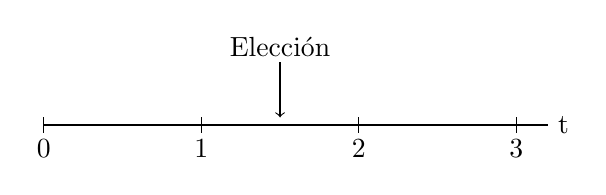
\begin{tikzpicture}
    % Dibuja la línea horizontal
    \draw[thick] (0,0) -- (6.4,0);
    % Marcas en la línea de tiempo
    \foreach \x in {0, 1, 2, 3} \draw (\x*2, 0.1) -- (\x*2, -0.1);
    % Puntos de tiempo
    \node at (0, -0.3) {0};
    \node at (2, -0.3) {1};
    \node at (4, -0.3) {2};
    \node at (6, -0.3) {3};
    \node at (6.6, 0) {t};
    % Etiqueta de Elección y flecha
    \node at (3, 1) {Elección};
    \draw[->] (3, 0.8) -- (3, 0.1);
\end{tikzpicture}
\end{center}
\end{document}
